On sait par définition que le delta d'un call européen vaut \[\Delta_{c}=\frac {\partial C}{\partial S}\]
Cette équation peut être approché par la méthode des différences finies centrées: \[\Delta_{DF}=\frac{C(S_{0} + \epsilon)-C(S_{0}-\epsilon)}{2\epsilon}\]

En utilisant la méthode de Black et Scholes on obtient un delta d’un call européen avec le paramètres suivants: $S_{0}$ = 75, le strike K=75, l’écheance T = 1, la volatilité  = 0.17 et le taux d’actualisation r = 0.01 qui vaut $\Delta_{B-S}$=0.5572.

Pour analyser l’influence de la profondeur de l’arbre, il faut donc calculer C(So+$\epsilon$) et C(So-$\epsilon$) à l’aide de la méthode de la Section~\ref{sec:question_3} afin d'obtenir par différences finies (avec $\epsilon$=0.001), le résultat voulu. On obtient les Figure~\ref{fig:delta_call_euro_df}, Figure~\ref{fig:delta_put_euro_df}. Cette formule a été implémentée dans la fonction Listing~\ref{listing:4}, et on peut la tester dans le fichier \textsc{delta.py}.




\begin{figure}[H]
\centering
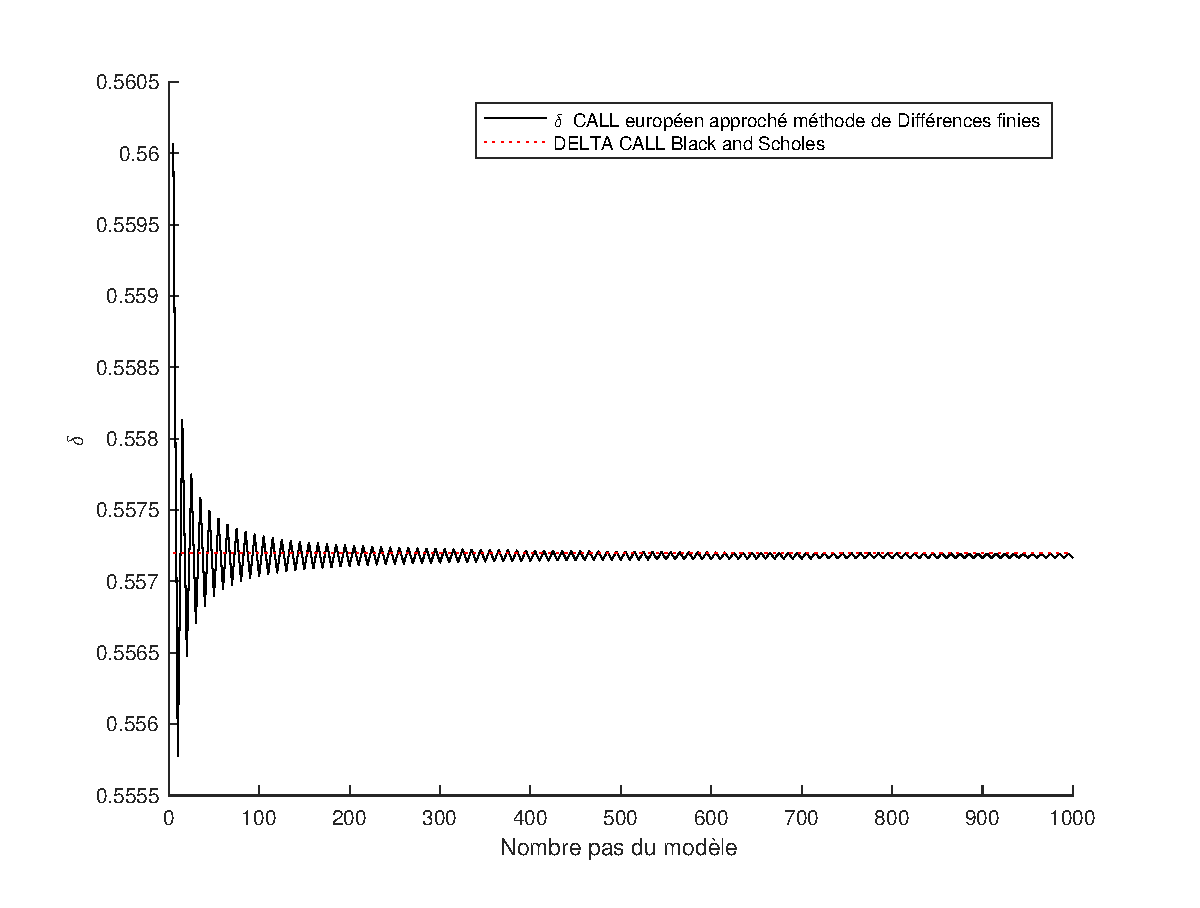
\includegraphics[scale=0.6]{./img/DELTA_CALL_EURO_DF-BS.eps}
\caption{Variation du $\delta$ d'un CALL européen approché par la méthode de différences finies en fonction du nombre de pas}
\label{fig:delta_call_euro_df}
\end{figure}

\begin{figure}[H]
\centering
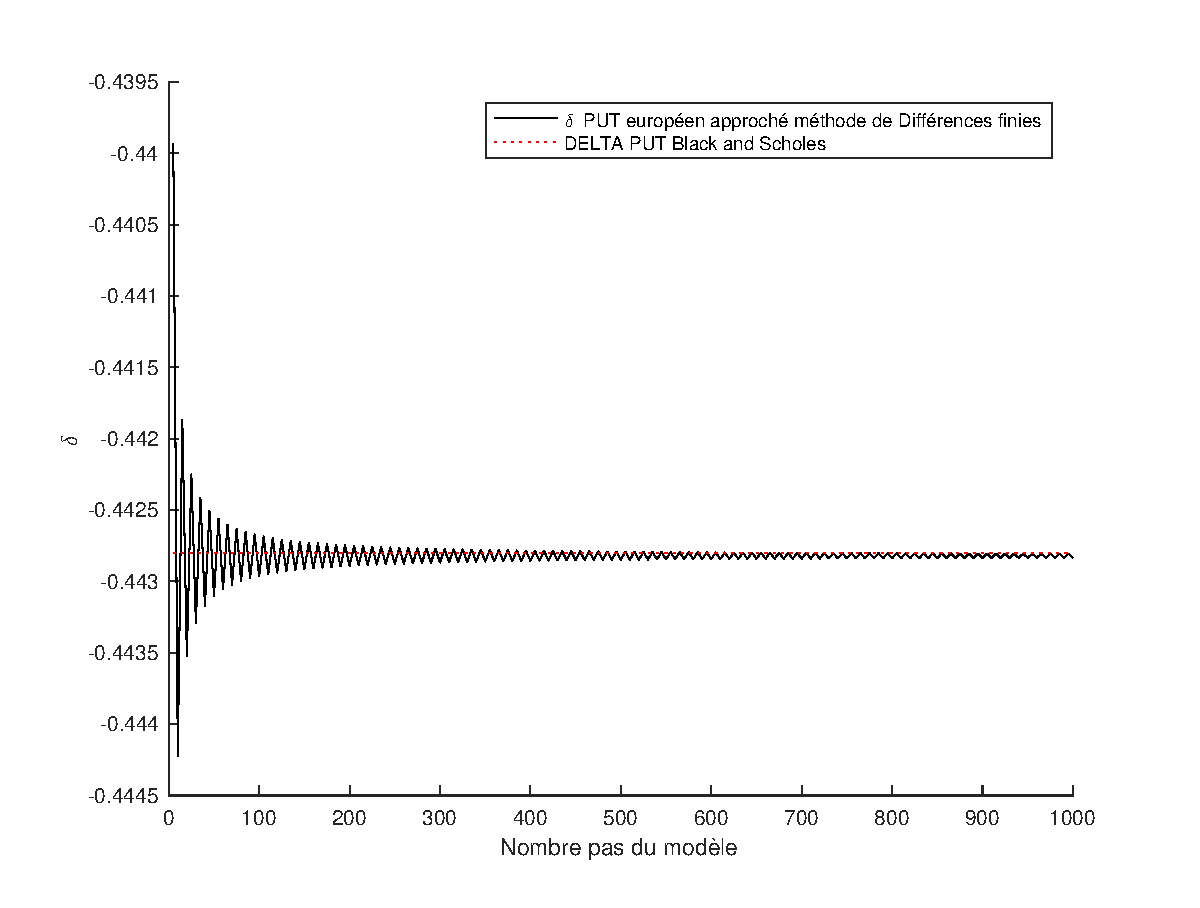
\includegraphics[scale=0.6]{./img/DELTA_PUT_EURO_DF-BS.eps}
\caption{Variation du $\delta$ d'un PUT européen approché par la méthode de différences finies en fonction du nombre de pas}
\label{fig:delta_put_euro_df}
\end{figure}

Il est clair que plus le nombre de pas augmente, plus l'amplitude de variation autour de $\delta$ diminue. De plus la vitesse de convergence est clairement rapide.